\documentclass{article}
\usepackage[utf8]{inputenc}
\usepackage{graphicx}
\usepackage{amssymb, amsmath, amsthm}
\usepackage{bbm}
\usepackage{biblatex}
\addbibresource{references.bib}
\newcommand\numberthis{\addtocounter{equation}{1}\tag{\theequation}}
\usepackage[margin=1in]{geometry}
\parskip = 0.1in

\begin{document}
\title{Forest Fires: An Analysis of the Initial Spread Index}
\date{December 12, 2017}
\maketitle
\begin{abstract}

\end{abstract}

\section{Introduction}

Forest fires ravage entire ecosystems and have lasting consequences on the environment beyond their path of destruction. These fires deplete oxygen from the atmosphere, impact the lumber industry, vanquish animal habitats, and damage areas of natural beauty. They also contribute to pollution, carbon emission, soil erosion, flooding, and water contamination. As our planet is increasingly threatened by rising temperatures and dangerous policies, it is imperative that we be more responsible with our resources. Statistics offers many tools that can reveal ways to be more mindful and efficient in addressing complex problems. Here, we will use the theory of linear modeling to analyze the initial spread of forest fires. In particular, we look to pick up where Smokey Bear left-off: the next line of defense after prevention is early-detection. By understanding the factors of initial spread, we hope to contribute to the fight against forest fires.

To accomplish this goal, we examine Initial Spread Index (ISI) as our response variable from data obtained in Monteshino Natural Park between 2000 and 2003. It is worth emphasizing that our target is not forest fire occurrences. This subtle difference goes against our intuition. For example, regarding the presence of people, we expect that the number of fires increases with the presence of people. On the other hand, more people means earlier detection. Therefore, we have no $\textit{a priori}$  knowledge of the relationship between people and ISI. This difficulty extends to other variables such as rain and wind, in which different arguments could be made to explain different possible relationship with ISI.

Our analysis takes a standard approach by first splitting our data into training and testing sets, then performing feature engineering and variable selection on our training set, fitting our various models, and finally evaluating these models on our testing set. While we do make predictions on the test set, our focus is on making statistically significant inferential conclusions. Therefore, we avoid using overly complicated transformations, and when faced with competing models, we select the simpler version. We understand that this may result in a sub-optimal predictive model, but our goal is to obtain interpretable coefficients and generalizable results. We chose this inferential approach because we believe the first step to combatting forest fires is understanding how they initially spread, and without an understanding, what good is a highly predictive model? Naturally we want to understand the likely causes of forest fires with a high ISI, of which we explore variables related to climate, time, location, and people.

This paper is organized as follows. In Section \ref{Background} we give a summary of our reference paper and restate our goal in this context. In Section \ref{Analysis} we outline our analysis, including our initial exploration of the data, all feature engineering and variable selection, and our final modeling decisions. In Section \ref{Prediction}, we apply our final model to our holdout set in order to make unbiased inferences. We conclude our project in Section \ref{Discussion} with a general discussion of our results. Finally, relevant R code may be found in the attached Appendix.

\section{Background}\label{Background}

\begin{itemize}

\item summary of reference paper
\item how data were collected
\item goal
\item restate prediction problem

\end{itemize}

\section{Modeling/Analysis}\label{Analysis}

\subsection{Exploratory Data Analysis}

\begin{itemize}

\item initial ideas: what should matter, types of covariates (spatial, temporal, index)
\item first plots
\item identify problems (colinearity, skewness)

\end{itemize}

\subsection{Feature Design}\label{Engineering}

\begin{itemize}

\item transformations
\item creations
\item One interesting feature class in this problem is geo-spatial. The raw data contains $X$ and $Y$ coordinates corresponding to a grid that has been overlaid on the map of Monteshino Natural Park. Each coordinate ranges from 1 to 9, therefore there are 81 total boxes in the grid. Of course, the first attempts at capturing any geo-spatial signal involved looking at the raw $X$ and $Y$ coordinates, as well as their interaction. Unfortunately, many of these boxes were sparse and the 81 degrees of freedom necessary for the raw grid were detrimental to the modeling process. Instead, we designed several features based on these values. This resulted in three candidate features. First, we created new coordinates $X2$ and $Y2$ that were created from the following algorithm
\begin{align*}
1&. \text{ sum the first row, last row, first column, last column} \\
2&. \text{ combine the row or column with the lowest sum with its neighboring row or column} \\
3&. \text{ repeat steps 1 and 2 until every box contains at least 1\% of the data}
\end{align*}
The algorithm was written under the belief that your neighbors are most similar to you and therefore should be the first candidates when grouping spaces together. Applying this algorithm, we reduced the number of boxes from 81 to 12. We note that $Y2$ only has two levels, which is unsurprising since Monteshino Natural Park is wider than it is tall. The other two engineered features integrated outside information. For these, we found a topographical map of Monteshino Natural Park on Google Maps and overlaid the original $X-Y$ grid.  The result is Picture \#\#\#. From this, we created $\textit{forest\_ind}$, which is a binary variable that takes the value 1 when the box is mostly covered in trees and 0 otherwise, and $\textit{grid\_group}$, which identifies five major mountain ranges and groups the boxes that cluster around these mountain ranges. Both of these variables are intuitively appealing, since obviously a forest fire needs trees and generally travelers hike and camp on a single mountain range.

\end{itemize}

\subsection{Variable Selection}

\begin{itemize}

\item FFMC
\item LASSO
\item tradeoff between interpretability for inference vs prediction
\item creation of competing models - with and without FFMC
\item The three engineered geo-spatial features from Section \ref{Engineering} were all considered as covariates. Unfortunately, none were selected during variable selection, as LASSO zeroed their coefficients are they were not significant under further scrutiny. However, we firmly believed that there should be signal from these geo-spatial features. Our next attempt was to fit a Mixed Model with $\textit{grid\_group}$ or $X2:Y2$ as the random intercepts. Again, this did not provide an improvement. Similarly, we tried weighting by the number of fires in $\textit{grid\_group}$ and $X2:Y2$ to no avail. We concluded that without further refinement or data collection, all of the geo-spatial signal was being picked up by the class of climate features, and therefore $X$, $Y$, and the derivative variables were discarded for our final model.

\end{itemize}

\subsection{Modeling}

\begin{itemize}

\item types of model we considered: weighted, mixed intercept, good ol lm
\item someone please bootstrap something
\item best 2 models
\item model comparison
\item our choice and why

\end{itemize}

\section{Prediction}\label{Prediction}

%\begin{itemize}
%\item apply best model to test set
%\item report diagnostics
%\item report p-values
%\item MSE or some loss function
%\item final inferences
%\end{itemize}

Finally, we turn our attention to  evaluating the weather only based model by using the holdout set.  We begin by fitting the chosen model for on the test set data, which comprises 30\% of the original data set. These estimates are reported in table \ref{Parameter Estimates}.  

\begin{table}
\centering
\begin{tabular}{ | l | c | c |}\hline
  Variable & Estimate & Standard Error \\ \hline
  Intercept & 1.31 & 0.24 \\
  Is Summer & 0.58 & 0.16 \\
  Wind & 0.079 & 0.029 \\
  Temperature & 0.045 & 0.012 \\
  Is Raining & -0.26 &   0.47 \\
  \hline
\end{tabular}
\caption{Final Parameter Estimates}
\label{Parameter Estimates}
\end{table}


As previously noted, the estimates from normal theory are close to the estimates from a bootstrap, so the 95\% confidence intervals are reported based assuming normal errors:
\begin{table}
\centering
\begin{tabular}{  | l | c | }\hline
  Variable & $95\%$  Confidence Interval \\ \hline
  Intercept & $(  0.84,1.79  )$ \\
  Is Summer & $( 0.26,0.90   )$\\
  Wind & $(  0.02,0.14  )$ \\
  Temperature & $(  0.02,0.07  )$ \\
  Is Raining & $(  -1.19,0.67  )$ \\
  \hline
\end{tabular}
\caption{Final Confidence Intervals}
\label{Confidence Intervals}
\end{table}
All the confidence intervals except for the binary Is Raining variable do not contain zero, so we conclude that they are all different than zero.
However, the Is Raining confidence interval does contain zero, so we do not conclude that the Is Raining variable is significantly different than zero.  We also note that the confidence interval is quite wide and there is a large standard error because there were only two data points with rain in the test set. While rain was uncommon in the training set, it was less sparse than in the test set, so it is difficult to make inference on such a variable. 
%Fix Up Graphics Path
%\begin{figure}
%\centering
%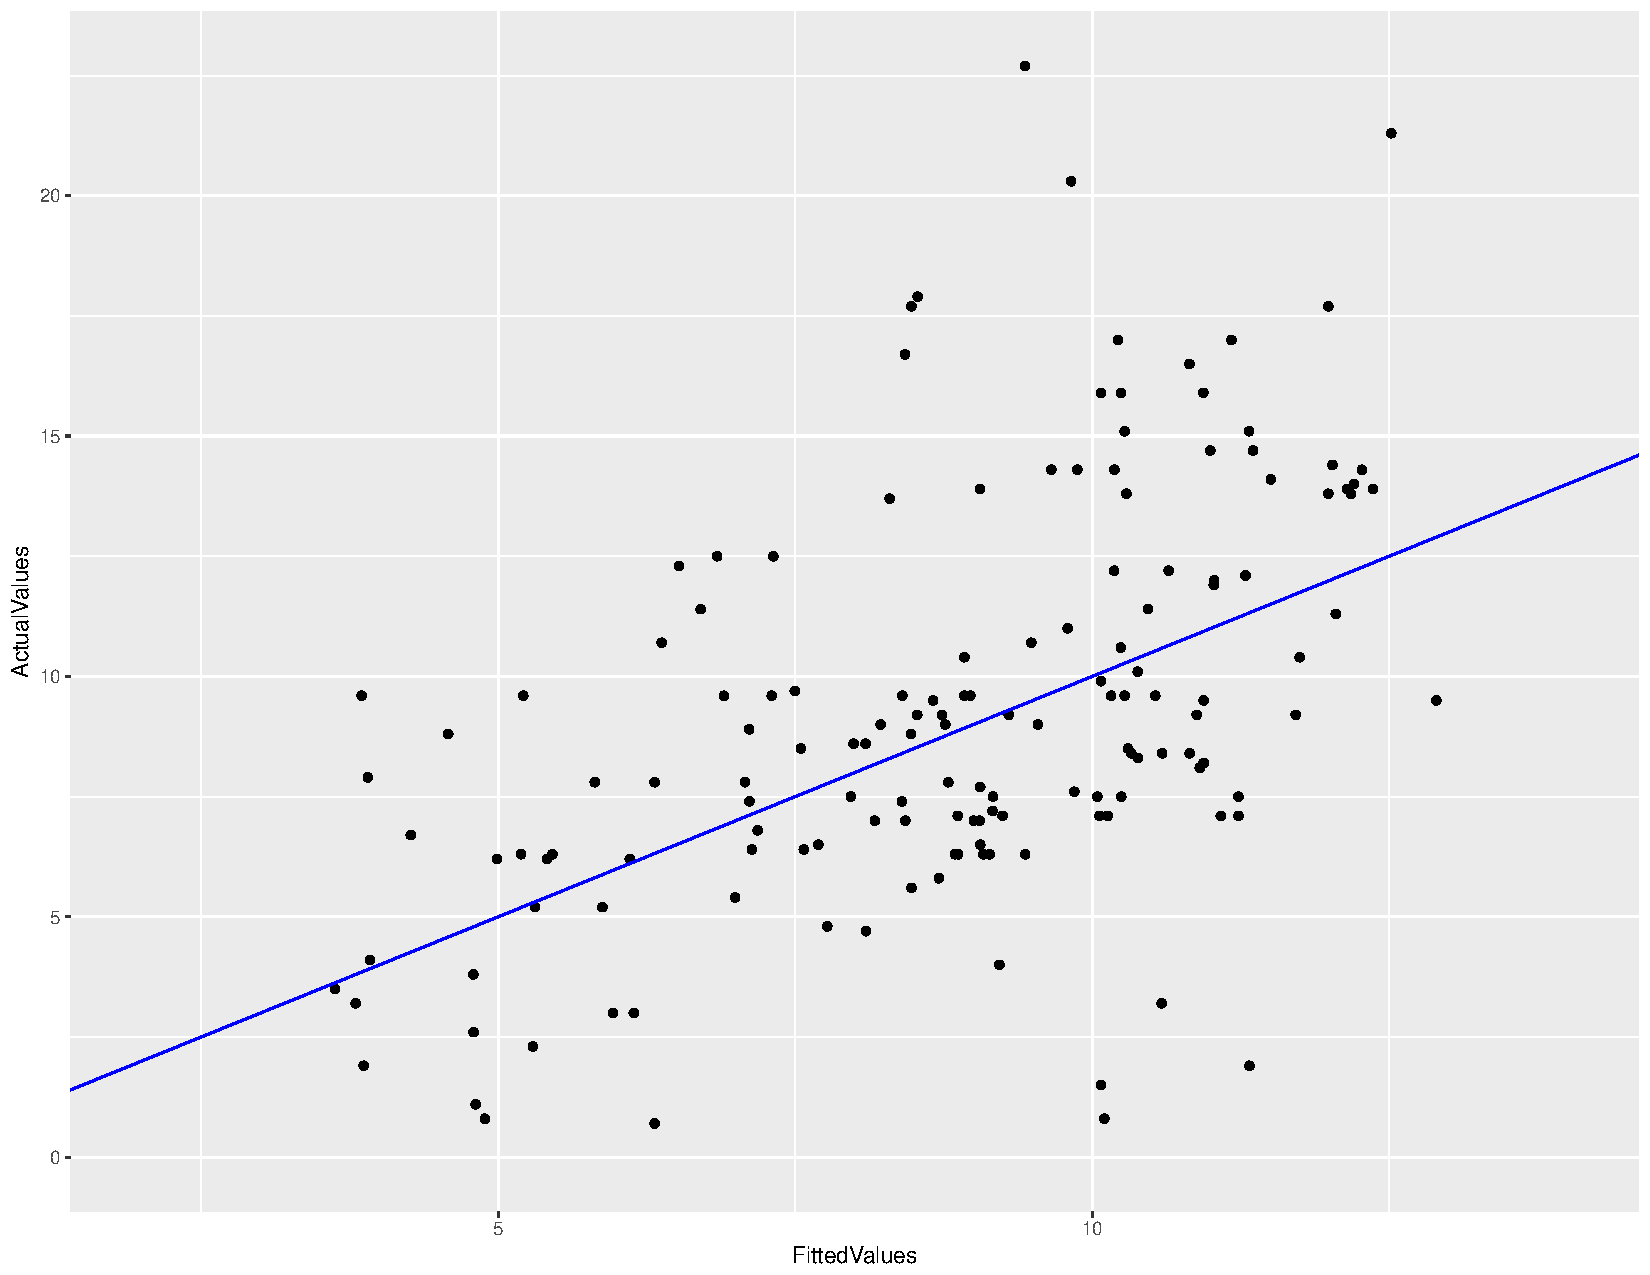
\includegraphics{TestSetFittedVsActual.pdf}
%\caption{Test Set Predicted vs Actual ISI}
%\label{TestSetPredictedVsActual}
%\end{figure}
By considering the predicted ISI values, the mean squared error was calculated to be $13.3$. 
%Fix Up Graphics Path
%\begin{figure}
%\centering
%\includegraphics{FinalModelDiagnostics.pdf}
%\caption{Test Set Diagnostics}
%\label{FinalModelDiagnostics}
%\end{figure}


The analysis on the test set mostly confirms the model selection performed on the training set, with the key difference being the loss of significance for the Is Raining variable.  We conclude that all weather variables except for rain impact the ISI, and fail to conclude that the presence of rain is a predictor for the model. The predictions from the model are reasonably close to the actual data based on an MSE criterion. 




\section{Discussion}\label{Discussion}

\section{Appendix}


\end{document}